\section{Problem Formulation}
  This section will presents the overall methodology of the study which will be devided into four parts.
  The conceptual of methodology is illustrated in Fig.~\ref{fig.method}.

  \begin{figure}[h!]
    \center
    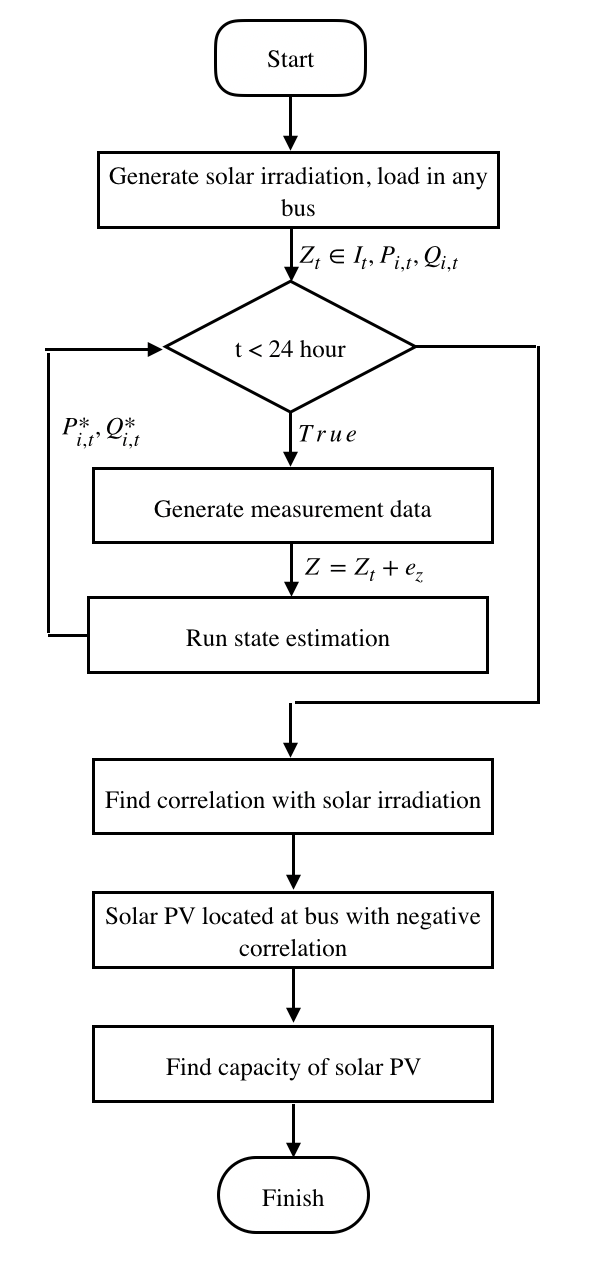
\includegraphics[scale=0.5]{images/conceptual_methodology.png}
    \caption{conceptual methodology}
    \label{fig.method}
  \end{figure}

  \subsection{Measurement devices, measured data and accuracy}
    In this study, there are three type of measurements; bus, line, and transformers measurement.
    Voltage magnitude in per unit is measurement at bus. Active and reactive power flow, and magnitude curreng are measured at line and trasformers.
    Bus measurement has 1$\%$ error and line measurement has 3$\%$ error.

    To generate measurement data for testing prurposes, measurement error was added to tha actual measurements as shown in Equation~(\ref{eq.Z}).
    \begin{equation}
      Z=Z_{a} \pm +e_{z}
    \label{eq.Z}
    \end{equation}
    where $Z_{a}$ is actual data and $e_{z}$ is error added base on accuarcy of the measurement.

    These error are assumed to be modeled independent Gaussian random variable\cite{b2}.
    where where the error value is expected value from gaussian distribution.
    noise is guassian distribution,as shown in Equation~(\ref{eq.gaussian}).
    \begin{equation}
      g(x)=\frac{1}{\sigma \sqrt{2\pi}}e^{-\frac{1}{2}((x-\mu)/\sigma)^2}
    \label{eq.gaussian}
    \end{equation}

  \subsection{Load allocation based state estimation}

    SE is based on the weighted least square (WLS) approach\cite{b1}.
    The method solves the following WLS problem to obtain an estimate ofthe system operating point defined by the system state x:
    \begin{equation}
      \underset{x}{min} J(x)=\sum_{i=1}^{m}w_{i}(z_{i}-h_{i}(x))^{2}=\big[ z-h(x)\big]^{T}W\big[z-h(x)\big]
    \label{eq.jacobian}
    \end{equation}
    where $w_{i}$ and $h_{i}(x)$ represent the weight and the measurements function associated with measurement $z_{i}$, respectively.
    For the solution of this problem the conventional iterative method is adape by solving following normal equations at each iteration, to compute the update $x^{k+1}=x^{k}+\Delta x^{k}$.

    \begin{equation}
      \big[ G(x^{k}) \big] \Delta x^{k} = H^{T}(x^{k})W \big[ z-h(x^{k}) \big]
    \label{eq.delta_x}
    \end{equation}

    Where

    \begin{equation}
      G(x)=H^{T}(x)WH(x)
    \label{eq.gain}
    \end{equation}

    is the gain matrix and H is the jacobian of the measurement function $h(x)$.

  \subsection{Solar PV site's location identification}

    This part will descript location identification of invisible solar PV's site.
    The correlation-based feature selection (CFS) is key tool here.
    The basis of the CFS that was introduced in \cite{b27}.
    The CFS will be peformed as a statistical measure of relationship between solar irradiation and load allocation from previous part.
    The measure is best used in these two variables that demenstrate a linear relationship between each other.
    The correlation coefficient that indicates the straength of the relationship between these two variables can be found using following formula:

    \begin{equation}
      \text{r}_{IP} =\frac{\sum(I_{i}-\overline{I})(P_{i}-\overline{P})}{\sqrt{\sum(I_{i}-\overline{P})^{2}(P_{i}-\overline{P})^{2})}}
    \label{eq.corr}
    \end{equation}

    where $\text{r}_{IP}$ is the correlation coefficient of the linear relationship between the solar irradiation (I) and load consumption (P),
    $I_{i}$ is the values of the solar irradiation variable in a sample, $\overline{I}$ is the mean of $I$,
    $P_{i}$ is the values of the load consumption variable in a sample, $\overline{P}$ is the mean of $P$.

    The negaive correlation shows that the variables tend to move in opposity directions (i.e., when one variable increases, the other variable decreases).
    The probability of solar PV site located at bus $i$ is expressed in Equation~(\ref{eq.prob_i})
    \begin{equation}
      \text{prob}_{i}= =
      \begin{cases}
        0 & \text{if  $r_{i}>=0$} \\
        1 & \text{if  $r_{i}<0$}
      \end{cases}
    \label{eq.prob_i}
    \end{equation}

  \subsection{Estimate solar PV site's installation capacity}

  Once, we can identify location of invisible solar PV located. Then, we try to estimate size of invisble solar PV units.
  We deploy change-point detection of change-point analysis.
  The change-point detection algorithm is a powerfull tools used to detect abrupt changes in time series data.
  We add solar irradiation and load allocation where invisble solar PV located. Then, we can find chaning point of the dataset.

  \begin{equation}
    \Delta D_{i,t} = p_{e}\Delta I_{i,t}
  \end{equation}
  where $p_{e}$ is the size of the unauthorized PV system at bus $i$, and time $t$.

  Then, we remove noise and find mean, range or other to estimate solar capacity.

  \subsection{Evaluation}
  This section will descripe evaluation methods will being used in this paper.
  There are two part of evaluate the proposed invisible solar PV size.
  First, the identification of the invisible solar PV location is evaluated by confusion matrix, $text{F}_1$ score, and Matthews correlation coefficient (MCC).
  Second, the estimation of installation of invisible solar PV size is evaluated by mean absolute error (MAE), and mean absolute percentage errot (MAPE).

  The results of location of invisible solar PV detection will be represented in confusion matrix as exampled in Table~\ref{tab.confusion_matrix}

  \begin{table}[ht]
    \caption{Confusion matrix}

  \begin{tabular}{cc|c|c|}
  \cline{3-4}
                                                                                                        &                                                                           & \multicolumn{2}{c|}{True condition}                                                                                           \\ \cline{2-4}
  \multicolumn{1}{c|}{}                                                                                 & Total population                                                          & Condition positive                                            & Condition negative                                            \\ \hline
  \multicolumn{1}{|c|}{\multirow{2}{*}{\begin{tabular}[c]{@{}c@{}}Prediction\\ condition\end{tabular}}} & \begin{tabular}[c]{@{}c@{}}Prediction\\ condition\\ positive\end{tabular} & \begin{tabular}[c]{@{}c@{}}True positive\\ (TP)\end{tabular}  & \begin{tabular}[c]{@{}c@{}}False positive\\ (FP)\end{tabular} \\ \cline{2-4}
  \multicolumn{1}{|c|}{}                                                                                & \begin{tabular}[c]{@{}c@{}}Prediction\\ condition\\ negative\end{tabular} & \begin{tabular}[c]{@{}c@{}}False negative\\ (FN)\end{tabular} & \begin{tabular}[c]{@{}c@{}}True negative\\ (TN)\end{tabular}  \\ \hline
  \end{tabular}
  \label{tab.confusion_matrix}
  \end{table}
  where TP, TN, FP, and FN are defined as number of hit, correct rejection, false alarm and miss, respectively.

  \subsubsection{$\text{F}_{1}$ score}
  The $\text{F}_{1}$ score is a measure of a test's accuracy.
  The $\text{F}_{1}$ score is the harmonic average of the precision and recall, where an $\text{F}_{1}$ score reaches its best value at 1 (perfect precision) and worst at 0.
  The $\text{F}_{1}$ is formulated in Equation~(\ref{eq.F_1_score}).
  \begin{equation}
    \text{F}_{1}=\frac{2\times \text{TP}}{2\times \text{TP} + \text{FP} + \text{FN}}
  \label{eq.F_1_score}
  \end{equation}

  \subsubsection{Matthews correlation coefficient}
  The Matthews correlation coefficient (MCC) is First introduced by biochememist Brian W. Matthews in 1975 \cite{b28}.
  The MCC is essence an correlation coefficient between theobserved and predicted binary classification; its returns a value between -1 and +1.
  A coefficient of +1 represetnes a perfection prediction, 0 no better than random prediction and -1 indicates total disagreement between prediction and observation.
  An Equation~(\ref{eq.MCC}) shows the formular of MCC for 2 classes. The dervations are express in \cite{b29}.
  \begin{equation}
    \text{MCC}=\frac{\text{TP} \times \text{TN} - \text{FP} \times \text{FN}}{\sqrt{(\text{TP}+\text{FP})(\text{TP}+\text{FN})(\text{TN}+\text{FP})(\text{TN}+\text{FN})}}
  \label{eq.MCC}
  \end{equation}

  \subsubsection{Mean absolute error and Mean absolute percentage error}
  The MAE defines as the difference between the actual and estimated invisible solar PV capacity which is computed by Equation~(\ref{eq.MAE}).
  The MAPE expresses the scaled difference between the actual and estimatedd invisible solar PV capacity as a percentage of the actual invisible solar PV capacity.
  MAPE is scale independent and it can be used to compare estimation performance across different data sets. MAPE can be calculated by Equation~(\ref{eq.MAPE}).

  \begin{equation}
    \text{MAE} = \frac{1}{N}\sum_{i=1}^{N} \left| p_{a}-p_{e} \right|
  \label{eq.MAE}
  \end{equation}

  \begin{equation}
    \text{MAPE} = \frac{100}{N}\sum_{i=1}^{N} \left| \frac{p_{a}-p_{e}}{p_{a}} \right|
  \label{eq.MAPE}
  \end{equation}

  where $p_{a}$ and $p_{e}$ are the actual and estimated solar PV installation capacity. $N$ is the number of sample.
